\question[10] Amir construye una casa para pájaros que parece un castillo. El diagrama muestra el techo de la casa.
Planea pintar de rojo el techo, pero necesita saber el área de la superficie para comprar la cantidad correcta de pintura,
como la que se muestra en la figura \ref{fig:prob_verb_superficie_06}.
\textbf{¿Cuál es el área de la superficie del techo, incluyendo la base?}

\begin{minipage}{0.3\linewidth}
    \begin{figure}[H]
        \begin{center}
            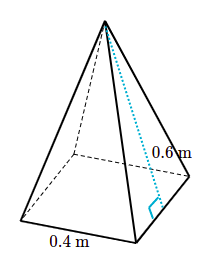
\includegraphics[width=0.8\textwidth]{../images/prob_verb_superficie_06}
        \end{center}
        \caption{}
        \label{fig:prob_verb_superficie_06}
    \end{figure}
\end{minipage}
\begin{minipage}{0.7\linewidth}
    \begin{solutionbox}{6cm}
        El volumen de un cilindro de radio $r$ y altura $h$ es:
        \begin{equation*}
            V = \pi r^2 h
        \end{equation*}
        De la figura \ref{fig:vol_area_03} se sabe que $r=2$ y $h=5$, entonces
        \begin{equation*}
            \begin{split}
                V & = \pi r^2 h\\
                & = \pi (4)^2 (10)\\
                & = \pi (16) (10)\\
                & = 160\pi
            \end{split}
        \end{equation*}
    \end{solutionbox}
\end{minipage}